\section{Analisi}
\label{sec:analisi}

\subsection{Package di analisi}

\diagramma[0.85\textwidth]{PKG_-_Analisi_e_progettazione.png}{Package di analisi}{fig:pkg}

A livello di analisi il sistema è diviso in tre package: \textbf{GestioneEventi} (l'evento e il catalogo), \textbf{GestioneUtenti} (clienti e cassieri) e \textbf{GestioneVendite} (biglietti, abbonamenti e titoli di accesso). GestioneVendite usa gli altri due, perché ogni biglietto si riferisce a un evento e appartiene, se bloccato o venduto, a un cliente.

\subsection{Classi di analisi}

Per ogni package si riporta il diagramma delle classi con gli attributi tipizzati e le associazioni con molteplicità; a questo livello non si indicano le operazioni.

\subsubsection*{GestioneEventi}
\diagramma[0.32\textwidth]{GestioneEventi.png}{Classi di analisi: GestioneEventi}{fig:ca-eventi}

\subsubsection*{GestioneUtenti}
\diagramma[0.75\textwidth]{GestioneUtenti.png}{Classi di analisi: GestioneUtenti}{fig:ca-utenti}
Cliente e cassiere sono specializzazioni di \code{User}; il cassiere ha in più il codice dipendente.

\subsubsection*{GestioneVendite}
\diagramma[0.85\textwidth]{GestioneVendite.png}{Classi di analisi: GestioneVendite}{fig:ca-vendite}
Biglietto e abbonamento sono due tipi di titolo di accesso (\code{Voucher}). Un evento ha uno o più biglietti, uno per posto; un biglietto può appartenere a un cliente; un abbonamento copre zero o più eventi.

\subsection{Diagrammi di sequenza}
\label{sec:sequenza}

Per ogni scenario si riporta un diagramma di sequenza. I messaggi corrispondono ai metodi reali del codice; i messaggi di ritorno sono tratteggiati. L'annullamento delle prenotazioni scadute, incluso da UC2 e UC3, è richiamato con un frammento \texttt{ref} che rimanda al diagramma di UC6.

\subsubsection{UC1 -- Consultazione eventi}
\diagramma[0.6\textwidth]{UC1_-_Consultazione_eventi.png}{Sequenza UC1 -- Consultazione eventi}{fig:sd1}
La vista chiede al controller \code{search_future_events()}, che delega al DAO \code{find_future_events()}; l'elenco ottenuto è mostrato al cliente.

\subsubsection{UC2 -- Selezione posti}
\diagramma[0.6\textwidth]{UC2_-_Selezione_posti.png}{Sequenza UC2 -- Selezione posti}{fig:sd2}
Alla scelta dell'evento il controller esegue prima l'annullamento delle prenotazioni scadute (\texttt{ref} UC6), poi legge i biglietti dell'evento. Quando il cliente seleziona i posti, la vista chiede il totale con \code{calculate_total(tickets, subscription)} e lo mostra.

\subsubsection{UC3 -- Acquisto titolo di accesso}
\begin{figure}[H]
\centering
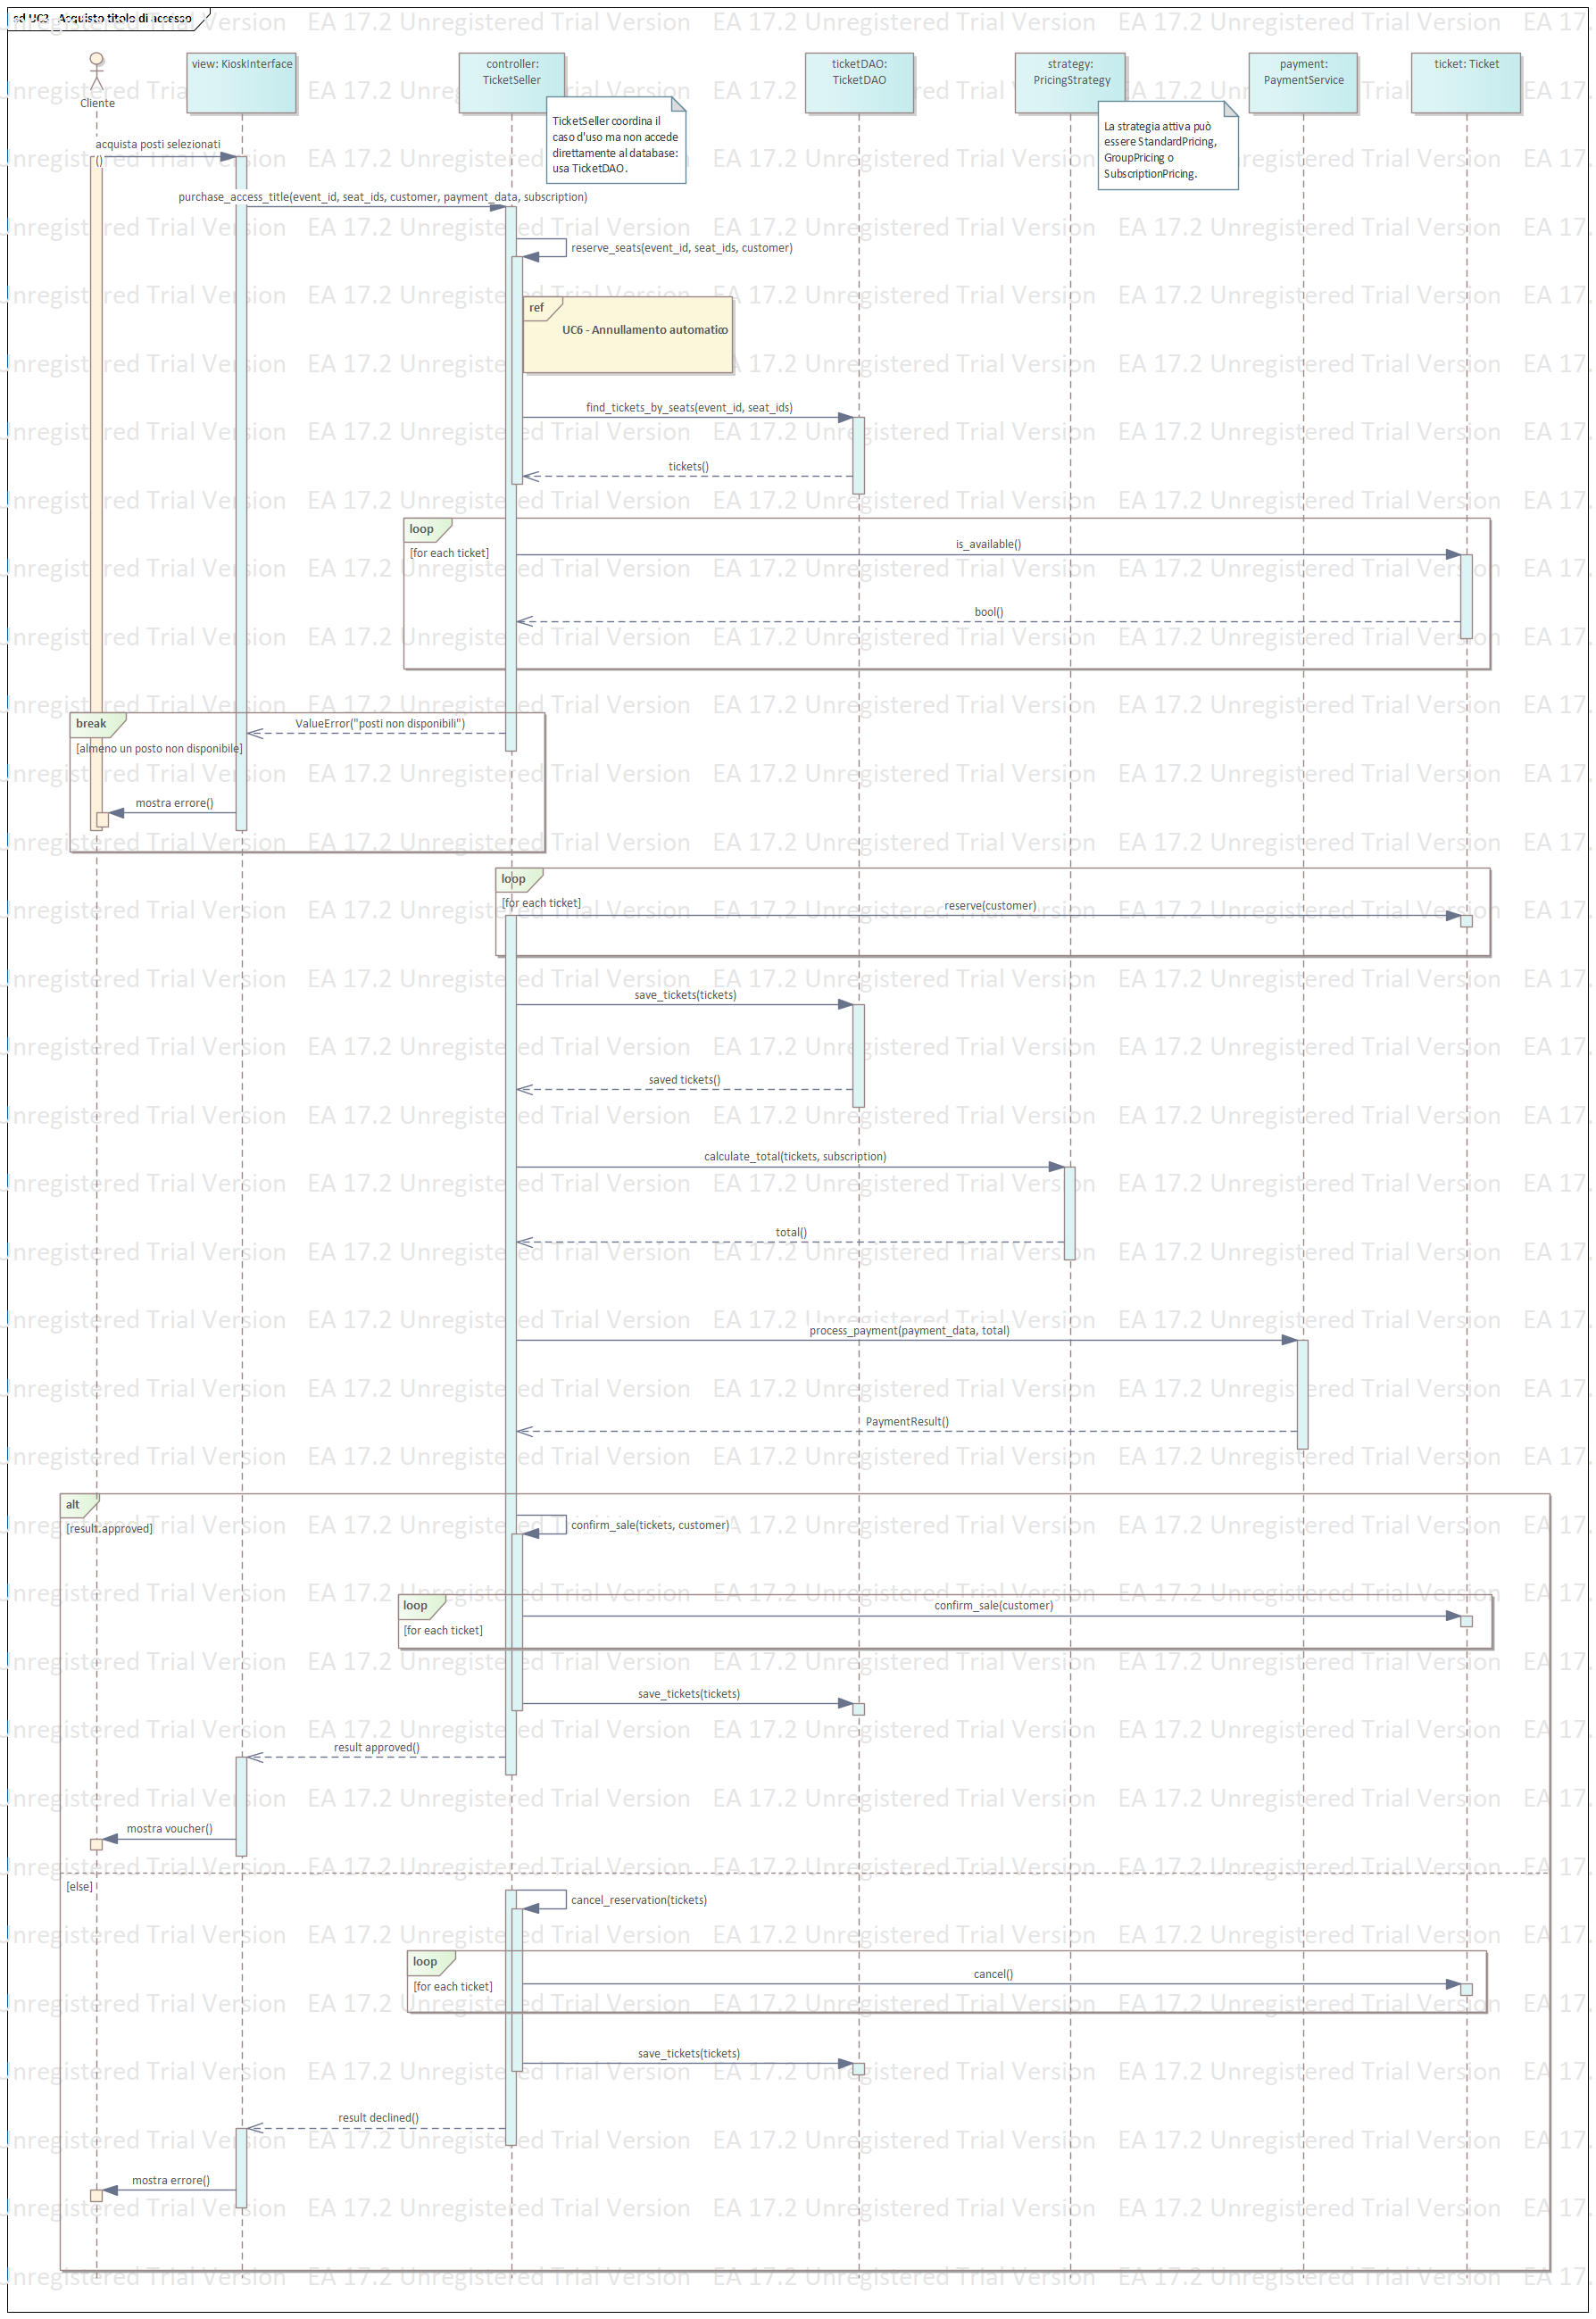
\includegraphics[height=0.88\textheight,width=\textwidth,keepaspectratio]{UC3_-_Acquisto_titolo_di_accesso.png}
\caption{Sequenza UC3 -- Acquisto titolo di accesso}
\label{fig:sd3}
\end{figure}
Il controller esegue \code{reserve_seats}: dopo l'annullamento delle prenotazioni scadute legge i biglietti e ne verifica la disponibilità. Se almeno un posto non è disponibile l'interazione termina con un errore (frammento \texttt{break}); altrimenti i biglietti sono bloccati e salvati, il totale è calcolato dalla strategia di prezzo e il pagamento è inviato al servizio esterno. Il frammento \texttt{alt} distingue il pagamento approvato (\code{confirm_sale} e codice della transazione) da quello rifiutato (\code{cancel_reservation} e messaggio di errore).

\subsubsection{UC4 -- Utilizzo abbonamento}
\diagramma[0.8\textwidth]{UC4_-_Utilizzo_abbonamento.png}{Sequenza UC4 -- Utilizzo abbonamento}{fig:sd4}
Il cliente inserisce il codice; la vista ottiene l'abbonamento con \code{find_subscription}. Quando l'abbonamento è presente il controller usa la strategia \code{SubscriptionPricing}, che sconta i biglietti degli eventi coperti.

\subsubsection{UC5 -- Gestione catalogo eventi}
\begin{figure}[H]
\centering
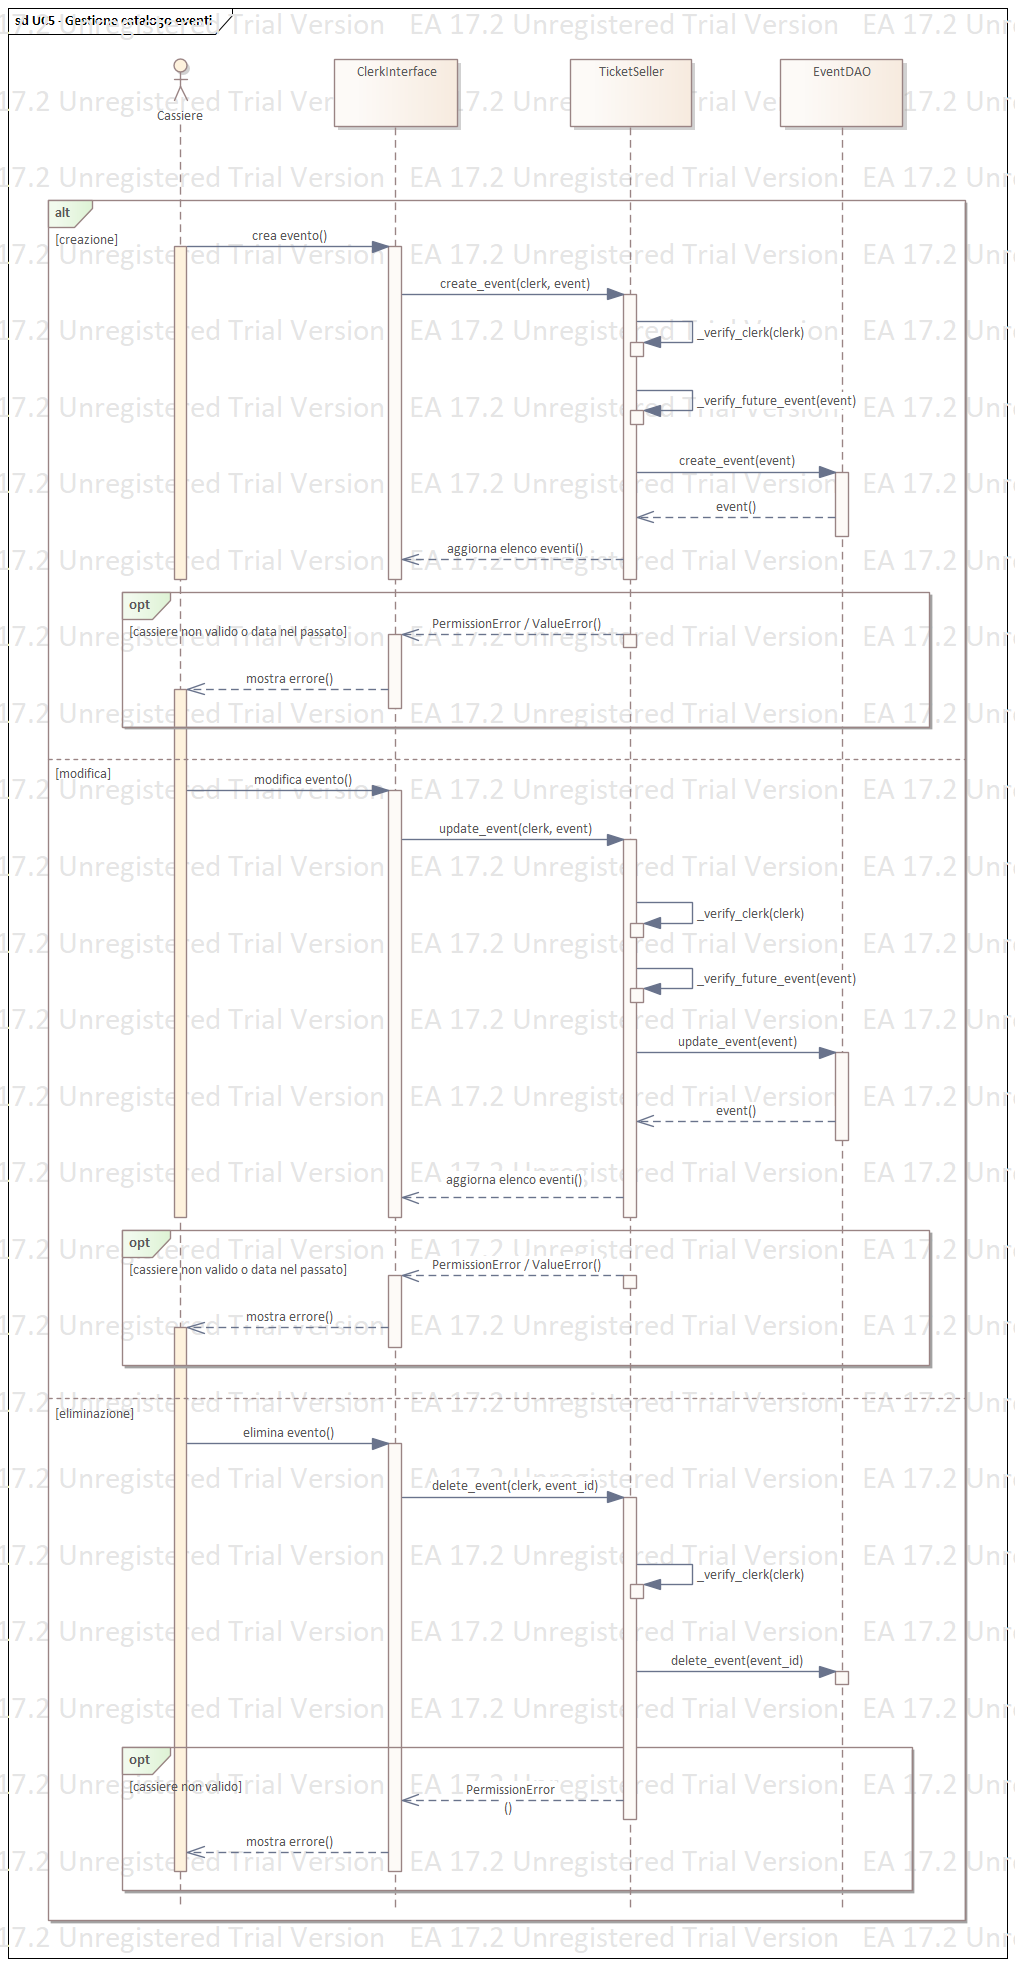
\includegraphics[height=0.88\textheight,width=\textwidth,keepaspectratio]{UC5_-_Gestione_catalogo_eventi.png}
\caption{Sequenza UC5 -- Gestione catalogo eventi}
\label{fig:sd5}
\end{figure}
Il frammento \texttt{alt} separa creazione, modifica ed eliminazione. In ogni ramo il controller verifica il cassiere (\code{_verify_clerk}) e, per creazione e modifica, la data futura (\code{_verify_future_event}), poi delega al DAO. Il frammento \texttt{opt} di ciascun ramo mostra il caso in cui un controllo non è superato: l'eccezione torna alla vista, che mostra l'errore.

\subsubsection{UC6 -- Annullamento automatico}
\diagramma[0.75\textwidth]{UC6_-_Annullamento_automatico.png}{Sequenza UC6 -- Annullamento automatico}{fig:sd6}
L'attore Tempo avvia \code{release_expired_reservations}: il controller legge i biglietti, annulla quelli bloccati da almeno 15 minuti e, se ce ne sono, li salva.

\subsection{Diagrammi di attività}
\label{sec:attivita}

Per ogni scenario si riporta un diagramma di attività con partizioni (chi esegue l'azione), nodi di decisione con guardie e nodi iniziale e finale.

\subsubsection{UC1 -- Consultazione eventi}
\diagramma[0.62\textwidth]{ACT_-_UC1_Consultazione_eventi.png}{Attività UC1 -- Consultazione eventi}{fig:act1}

\subsubsection{UC2 -- Selezione posti}
\diagramma[0.68\textwidth]{ACT_-_UC2_Selezione_posti.png}{Attività UC2 -- Selezione posti}{fig:act2}

\subsubsection{UC3 -- Acquisto titolo di accesso}
\diagramma{ACT_-_UC3_Acquisto_titolo_di_accesso.png}{Attività UC3 -- Acquisto titolo di accesso}{fig:act3}
Il cliente sceglie evento e posti, vede il totale, inserisce i dati di pagamento e conferma. Il sistema rilascia le prenotazioni scadute e controlla la disponibilità: se un posto non è disponibile mostra un errore, altrimenti blocca i posti, calcola il totale e invia il pagamento. In base all'esito conferma la vendita o annulla il blocco; in entrambi i casi salva i biglietti e mostra il risultato.

\subsubsection{UC4 -- Utilizzo abbonamento}
\diagramma[0.62\textwidth]{ACT_-_UC4_Utilizzo_abbonamento.png}{Attività UC4 -- Utilizzo abbonamento}{fig:act4}

\subsubsection{UC5 -- Gestione catalogo eventi}
\diagramma{ACT_-_UC5_Gestione_catalogo_eventi.png}{Attività UC5 -- Gestione catalogo eventi}{fig:act5}
Dopo la scelta dell'operazione il controller verifica il cassiere e, per creazione e modifica, la data dell'evento; se un controllo fallisce il flusso confluisce nel ramo di errore, altrimenti il DAO esegue l'operazione e la vista aggiorna l'elenco.

\subsubsection{UC6 -- Annullamento automatico}
\diagramma[0.85\textwidth]{ACT_-_UC6_Annullamento_automatico.png}{Attività UC6 -- Annullamento automatico}{fig:act6}
Il ciclo esamina un biglietto alla volta: se è bloccato e il blocco dura da almeno 15 minuti lo annulla e lo aggiunge alla lista dei rilasciati. Finiti i biglietti, la lista viene salvata solo se non è vuota.
